\begin{frame}
    \frametitle{Cámara de luz estructurada}
    \scriptsize
    \begin{center}
        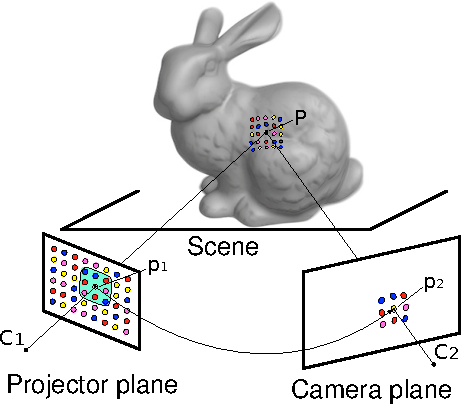
\includegraphics[width=0.3\columnwidth]{images/structured_light.pdf}
    \end{center}

    \begin{block}{Principio de funcionamiento}
        La luz estructurada (\emph{structured light}) es el proceso de proyectar un patrón conocido de píxeles (ocasionalmente rejillas o barras horizontales) en una escena. La manera en que dicho patrón se deforma cuando golpea distintas superficies permite a los sistemas de visión calcular la profundidad e información de la superficie de los objetos en la escena.
    \end{block}

    \begin{itemize}
        \item Exteroceptivo
        \item Activo
        \item No funcionan bien en entornos exteriores
        \item Corto Alcance
    \end{itemize}

\end{frame}